\chapter{Experimental setup and results}

The three self-supervised learning techniques mentioned were used in this study based on recommendations from the relevant research papers and with some customization. After training and evaluating these models using a linear evaluation protocol, it is concluded that the \gls{simclr} model outperforms the other methods mentioned given the setup. The following sections describe the model hyperparameter customizations, image transformations used, and a comparative analysis of the results.

\section{Model Configuration and Customizations}

The \gls{simclr} model includes erosion, dilation and random erasing in addition to transformations from Ying Chen et al. \cite{chen_simple_2020}. Each transform was applied randomly with a probability of 0.5. A kernel size of 5 is utilized for dilation while a kernel size of 3 is employed for erosion. An identical approach was used in \gls{byol} for preprocessing. The model configuration and hyperparameters passed for all the models are defined in \cref{tab:model-config}.

\begin{table}[ht]
	\begin{center}
            \caption{Pre-training configuration.}
		\resizebox{\textwidth}{!}{
			\begin{tabular}{@{}ll|ll|ll@{}}
				\toprule
				\multicolumn{2}{c|}{SimCLR}              & \multicolumn{2}{c|}{MAE}                       & \multicolumn{2}{c}{BYOL}                            \\ \midrule
				Variable           & Value               & Variable           & Value              & Variable           & Value             \\ \midrule
				Optimizer          & Adam                & Optimizer          & AdamW              & Optimizer          & Adam              \\
				Base learning rate & 1.5e-3              & Base learning rate & 3e-4               & Base learning rate & 3e-1              \\
				Weight decay       & 1e-6                & Optimizer momentum & $\beta_1=0.9, \beta_2=0.95$  & Weight decay       & 1.5e-6            \\
				Batch size         & 256                 & Weight decay       & 5e-2               & Target decay rate  & 0.996             \\
				Scheduler          & LambdaLR            & Scheduler          & Half-cycle cosine  & Batch size         & 64                \\
				Scheduler Function & Linear warmup decay & Batch size         & 512                & Scheduler          & Cosine annealing  \\
				Warmup Epochs      & 10                  & Warmup Epochs      & 10                 & Warmup Epochs      & 10                \\
				Loss function      & NT-Xent             & Loss function      & MSE                & Loss function      & Cosine similarity \\
				Temperature        & 0.1                 & Backbone           & Vision Transformer & Backbone           & ResNet-50         \\
				Backbone           & ResNet-50           &                    &                    &                    &                   \\ \bottomrule
			\end{tabular}
		}
		\vspace{5pt}
		\label{tab:model-config}
	\end{center}
\end{table}

Evaluation of multiple \gls{vit} block sizes for backbone architecture in \gls{mae} revealed that ViT-Large demonstrated superior performance in terms of learning and numerical stability. Whereas, both ViT-Base and ViT-Huge consistently resulted in \gls{nan} loss, while ViT-Tiny proved to be insufficient to learn features. Whereas, the added Erosion and Dilation augmentations to SimCLR were not performing well. Furthermore, extensive experimentation revealed that a large batch size of 512 and a learning rate scheduler are crucial for attaining good training results.

\section{Pre-training progress and monitoring}

The self-supervised methods in this study are pre-trained on the \gls{icdar}-\gls{clamm} dataset, which encompasses 12 classes for script type classification. To ensure consistency and reproducibility, a deterministic train, validation, and test split is performed, with a ratio of 70:10:20 percentages and a seed of 42. The test set remains untouched and is reserved for subsequent evaluation.

The models are pre-trained for a total of 500 epochs. The choice of a larger number of epochs is driven by the fact that the models are trained from scratch. This extended training duration allows the models to learn meaningful representations and capture intricate patterns present in the dataset.

By utilizing the powerful computational capabilities of \glspl{gpu} and parallel data loading to accelerate the training process, resulting in the convergence of the models over 500 epochs. Over 150 experiments were conducted with varying configurations to find optimal parameters for convergence.

\begin{figure}[ht]
	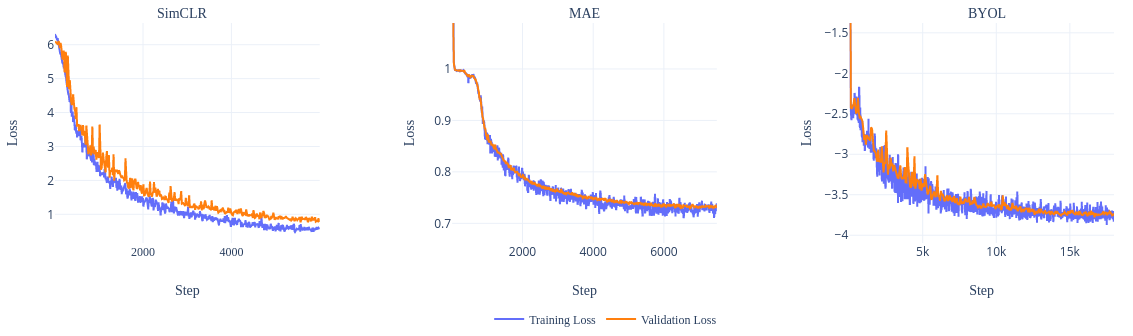
\includegraphics[width=\textwidth]{all_loss_curves.png}
	\centering
	\caption[Pre-training loss curves]{Loss curves for pre-trained models with batch size of 256, 256 and 64 from left to right.}
	\label{fig:loss}
\end{figure}

Throughout the pretraining process, periodic evaluations are conducted to monitor the models’ progress. Metrics such as training loss, validation loss, and grad norm are measured to assess the performance of the models at different stages of training. The loss curves for the best performing model generated during pre-training are shown in the \cref{fig:loss}. These metrics played a crucial role in identifying and mitigating \gls{nan} loss caused by the issues of vanishing and exploding gradients.

\begin{figure}
	\centering
	\begin{subfigure}[b]{0.3\textwidth}
		\centering
		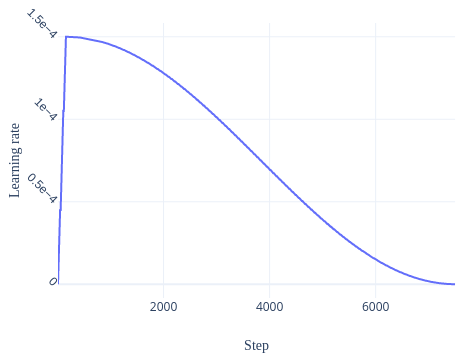
\includegraphics[width=\textwidth]{cosine_lr_sched.png}
		\caption{Learning rate}
	\end{subfigure}
	\hspace{10pt}
	\begin{subfigure}[b]{0.3\textwidth}
		\centering
		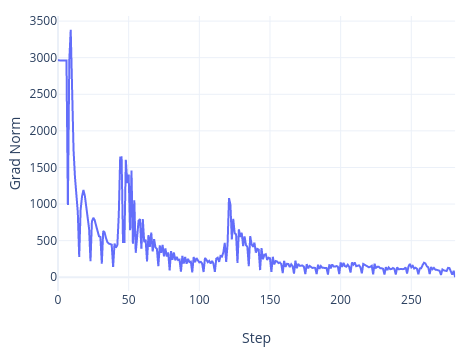
\includegraphics[width=\textwidth]{grad_norm.png}
		\caption{Normalized gradient}
	\end{subfigure}
	\caption[Metrics monitored for MAE]{Metrics for MAE (a) Half-cycle cosine learning rate decay after warmup. (b) Normalized gradient after each step.}
    \label{fig:lr_sched_grad}
\end{figure}

\section{Performance Evaluation}

In order to assess the effectiveness of the learned representations through transfer learning, a downstream task of script type classification is performed using the pre-trained models. This evaluation serves to gauge the transferability and generalization capabilities of the representations acquired during the self-supervised pretraining phase.

\subsection{Evaluation Metric}

To assess the quality and transferability of the learned representations, a linear evaluation protocol is employed. This evaluation protocol serves as a standardized framework for evaluating the performance of the pre-trained models on a downstream task \cite{kocaman_saliency_2022}. During the linear evaluation, the accuracy metric is employed to measure the performance of the linear classifier on the script type classification task. These metrics provide a quantitative assessment of the models’ ability to generalize and make accurate predictions in the specific task context.

In addition, to acquire insights into the class distribution and the quality of the learned embeddings, a visualization technique based on \acrfull{tsne} is employed. \gls{tsne} provides a powerful visualization method for exploring high-dimensional data by reducing its dimensionality while preserving the underlying structure \cite{maaten_visualizing_2008}.

\begin{figure}[ht]
	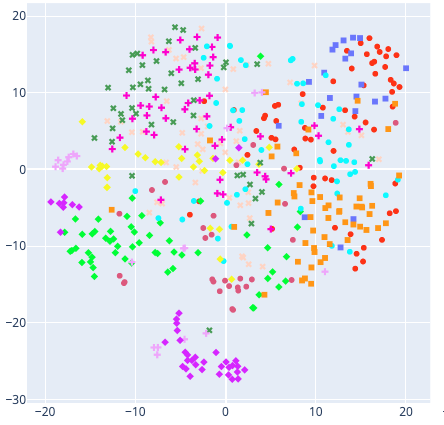
\includegraphics[width=0.45\textwidth]{simclr_embed_visualization.png}
	\centering
	\caption{t-SNE visualization of embeddings with 12 classes for SimCLR}
	\label{fig:figure}
\end{figure}


\subsection{Quantitative Results}

In this section, the results from the evaluations are presented and compared. The evaluation results for all the models are displayed in the \cref{tab:eval}. It is evident that, with a linear evaluation accuracy of 71.8\% \gls{simclr} outperforms \gls{mae} and \gls{byol}. 

\begin{table}[ht]
\begin{center}
\caption{Evaluation results.}
\begin{tabular}{@{}l|cc|cc@{}}
\multicolumn{1}{c|}{}       & \multicolumn{2}{c|}{Pre-training} & \multicolumn{2}{c}{Linear Evaluation}                                                                                 \\ \midrule
\multicolumn{1}{c|}{Model Name} & Epochs        & Batch size        & \begin{tabular}[c]{@{}c@{}}Training \\ epochs\end{tabular} & \begin{tabular}[c]{@{}c@{}}Top-1\\ accuracy\end{tabular} \\ \midrule
SimCLR                      & 500           & 256               & 100                                                        & 71.8\%                                                   \\
MAE                         & 500           & 256               & 100                                                        & 36.1\%                                                   \\
BYOL                        & 500           & 64                & 100                                                        & 45.2\%                                                  
\end{tabular}
\label{tab:eval}
\end{center}
\end{table}

It is worth noting that \gls{mae} with a \gls{vit} backbone shows a lower accuracy of 36.1\%. This observation can be attributed to its higher data requirements, as \gls{mae} with \gls{vit} demands a larger dataset for effective pre-training. The lower accuracy suggests that the available dataset size might not have been sufficient to fully leverage the potential of the \gls{mae} model with a \gls{vit} backbone. These findings highlight the importance of the choice of model architecture and the impact it has on the performance of downstream tasks given the complexity of the dataset. \gls{simclr}’s success can be attributed to its ability to learn robust representations even with a comparatively smaller dataset.

\subsection{Computational Efficiency}

The models performance differs in terms of trainable parameters, pre-training time, checkpoint size for the same GPU acceleration. \gls{simclr} has the fewest parameters and the smallest checkpoint size, while \gls{mae} has the shortest pre-training time and the largest parameters. This indicates that \gls{simclr} is the least complex of all. Consideration of these factors can be crucial in selecting the most suitable model based on the available computational resources.

Furthermore, the implementation of effective learning techniques like gradient accumulation proved to be useful in training models with bigger batch sizes that exceed the memory capacity limitation of \glspl{gpu}. \cref{tab:computational} presents a comprehensive analysis of the metrics that impact computational efficiency, allowing for easy comparison. 


\begin{table}[ht]
\begin{center}
\caption{Comparison of computational efficiency metrics for models trained for 500 epochs.}
\begin{tabular}{@{}l|c|c|c|c@{}}
\multicolumn{1}{c|}{Model Name} & \begin{tabular}[c]{@{}c@{}}Trainable Params \\ (millions)\end{tabular} & \begin{tabular}[c]{@{}c@{}}Pre-training Time\\ (hours)\end{tabular} & GPU      & \begin{tabular}[c]{@{}c@{}}Checkpoint Size\\ (MB)\end{tabular} \\ \midrule
SimCLR                          & 30                     
& 4.3                                                                 & 1 x A100 & 329                                                            \\
MAE                             & 329                                                                    & 2.61                                                                & 1 x A100 & 3700                                                           \\
BYOL                            & 68                                                                     & 5.06                                                                & 1 x A100 & 528                                                           
\end{tabular}
\label{tab:computational}
\end{center}
\end{table}